% Selected DSN2027 manuscript; evidence and release provenance are archived separately.
\documentclass[conference,10pt]{IEEEtran}
\usepackage[T1]{fontenc}
\usepackage{cite,amsmath,amssymb,amsthm}
\usepackage{booktabs,array,multirow,graphicx}
\usepackage{url,microtype}
\usepackage[hidelinks]{hyperref}
\newtheorem{definition}{Definition}
\newtheorem{proposition}{Proposition}
\begin{document}
\title{RevTrace: Preserving Valid Progress across Trusted Feedback Revisions}
\author{\IEEEauthorblockN{Anonymous submission}\IEEEauthorblockA{Regular paper}}
\maketitle
\begin{abstract}
Trusted feedback can withdraw a timely transcript even when its
computation remains valid. RevTrace preserves such progress by separately
confirming complete call inputs, retaining original selection authority,
and checking support for the Consumer's whole view. A conditional call
can remain eligible even when its own next prediction is wrong; an
accepted result can outlive its producer. A selected-trace refinement
argument connects this coordination to the protected program. In a
predeclared 24-speaker stratum, computation retention alone increases
frontier withdrawals from 12 to 17; joint retention yields zero and adds
26.645 seconds of deadline credit over 714.110 seconds offered. In a
matched native correction study, the final protocol preserves original
histories, delivers 65.822 of 66.340 deadline-credited seconds, and passes
both whole-run deadlines in six of eight trials, versus none for
conservative execution. Fault and sustained-state tests expose recovery,
quality, and resource boundaries.
\end{abstract}
\begin{IEEEkeywords}
dependable inference, feedback state, incremental computation, speculative execution, streaming ASR
\end{IEEEkeywords}
\section{Introduction}\label{sec:intro}
A streaming transcript can arrive on time and still disappear when trusted
feedback advances. In one actual run, a complete two-second audio interval
introduced 37 visible characters at 1.444~s, within its two-second display
deadline. A trusted update at 1.544~s replaced that whole hypothesis with
a shorter snapshot, although its computation remained compatible with the
selected feedback state. Identical text returned through certified
delivery at 3.720~s, within the eight-second deadline. Both first-delivery
obligations were met, yet the phrase was absent for 2.176~s, including at
the original display deadline (Figure~\ref{fig:continuity_case}). The
service lost delivered progress without needing to correct it. Trusted
feedback here means feedback accepted by protected selection.

\begin{figure*}[t]
\centering
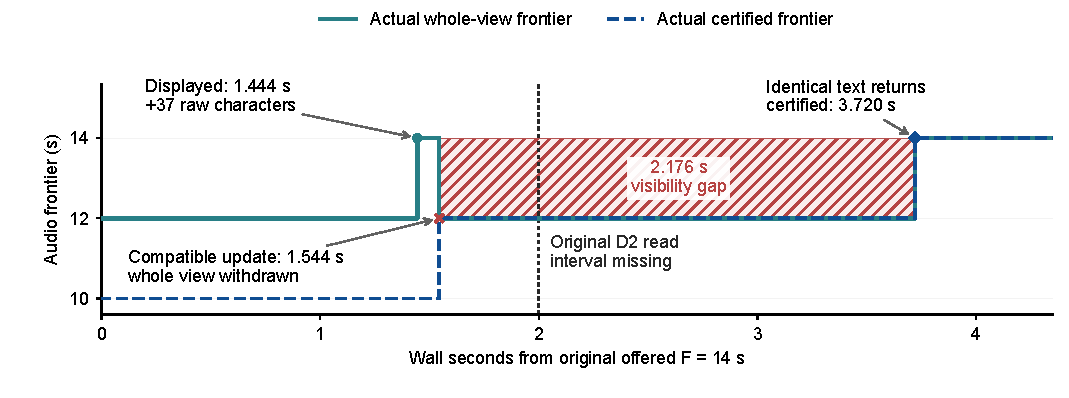
\includegraphics[width=\textwidth]{figures/timely_full_interval_case.pdf}
\caption{Timely first delivery can still leave a gap in delivered progress.
An actual computation-only run displays a complete interval at 1.444~s,
withdraws it under a compatible update at 1.544~s, and restores identical
text at 3.720~s. Shading marks the 2.176-s gap; the vertical line is the
original D2 read point. The view introduces 37 raw code points including
spaces, not character/audio alignments. This c16 overload case illustrates
the failure mode, not its incidence or a whole-run service win.}
\label{fig:continuity_case}
\end{figure*}

This problem arises when generated or corrected output becomes an input
to subsequent inference. Streaming speech correction is a concrete case:
StreamCorrect feeds its chosen correction into later recognition
\cite{vu2026streamcorrect}. A new trusted selection can invalidate some
speculation while confirming other work that began earlier. Recomputing
everything is conservative, but retaining computation alone is also
insufficient. In our predeclared 24-speaker evaluation, computation
retention improves timely delivery while increasing audio-frontier
withdrawals from 12 to 17. Jointly retaining computation and its supported
whole view yields zero. The missing obligation is to turn valid work into
\emph{sustained service} across a trusted revision.

Three questions determine the actions. Does an old call's complete frozen
input still match the selected parent feedback state? Has the original selection
authorized its result? Does the Consumer's current whole hypothesis still
have a complete dependency path from that parent? These questions concern
different objects. A call can have a confirmed input while its own next
prediction is wrong. A view can lose support while a future call's input
is unresolved. A producer can die after its complete result has already
been accepted. A birth version, matching text, or producer-liveness bit
cannot stand in for all three judgments.

RevTrace checks complete frozen inputs and dependency paths before
retaining work, leaves result selection to the original program, and
revalidates the Consumer's entire displayed hypothesis when a selected
state installs.
Incremental dialogue and computation supply established dependency and
revocation principles~\cite{schlangen2011incremental,hammer2014adapton,hammer2015names}.
SSBD already combines draft reuse and display masking
\cite{zeng2026ssbd}; PredGen speculates across evolving speech stages
\cite{li2025predgen}. Our focus is a recursively selected feedback task:
retained work must still execute its original correction and update, and
applying a new selected root must separately validate the actual whole
view. The contribution is this concrete coordination contract and its
service consequences, rather than reuse or revocation in isolation.

We make three contributions:
\begin{itemize}
\item We identify a service gap between timely first delivery and continued
  availability under compatible feedback, and define executable witnesses
  for complete-call eligibility and whole-view retention
  (Sections~\ref{sec:contract}--\ref{sec:continuation}).
\item We implement their joint coordination with original selection,
  durable facts, and physical ownership. A conditional selected-trace
  refinement argument explains how early full calls preserve the protected
  task, including accepted results across supported process failures
  (Sections~\ref{sec:continuation}--\ref{sec:protocol}).
\item We test the composition on real neural service: factorial controls
  isolate the interaction, native correction tests original full calls,
  and fault and sustained-state controls establish its costs and limits
  (Section~\ref{sec:eval}).
\end{itemize}

Deadline credit counts offered audio seconds meeting both first-display
and certified-delivery deadlines. The headline joint arm adds 26.645~s over
714.110~s offered with unchanged selected histories. A matched native
comparison raises credit from 30.0 to 65.822 of 66.340~s and whole-run
passes from zero to six of eight; resident independent requests pass
seven of eight. The remaining EOS misses, overload, cold recovery, and
no-reset quality failures delimit the service claim.

\section{Feedback Contract}\label{sec:contract}
\subsection{Feedback creates an execution dependency}
An immutable audio stream supplies a protected selection path producing
\emph{Canonical} facts and a faster \emph{Private} path computing and
displaying provisional hypotheses. Selection can change the next call's
input: StreamCorrect feeds its chosen correction into subsequent
ASR~\cite{vu2026streamcorrect}. We coordinate this dependency as the paths
advance asynchronously.

For a fixed session and execution contract, write an installed fact as
\begin{equation}
 C=(v,F,Z_C,P_C,T_C).
 \label{eq:canonical}
\end{equation}
Here $v$ is the version, $F$ the certified processing frontier, $Z_C$ the
complete selected output, $P_C$ the feedback state, and $T_C$ its bound
text. The contract fixes the model, adapter, decoding, audio identity,
and transformations to $P$ and $T$. Consumer coverage follows the adapter's
publication policy; advancing $F$ need not add characters. Certification
means acceptance by protected selection and installation, separately
from human-transcription accuracy.

The adapter declares a conservative representation of \emph{all mutable
cross-call state that can affect later model inputs, selection, or feedback}.
Telemetry and resources are separate. Qwen passes prompt tokens without
cross-call numerical KV caches. The native adapter additionally carries
audio buffers, token groups, context, alignment position, and decoder
configuration. Comparisons require the same contract: text equality
cannot replace an omitted cursor or numerical cache. The representation
may conservatively include fields unnecessary to a particular call.

\subsection{Three lifetimes of provisional work}
A complete provisional node $n$ records a frozen call
\begin{equation}
 q_n=(a_n,P_n^-,b_n,\chi_n),\quad
 n=(q_n,Z_n,P_n^+,T_n),
 \label{eq:node}
\end{equation}
where $a_n$ is the input-state frontier, $b_n>a_n$ the audio target, and
$\chi_n$ binds remaining inputs and execution identity. The model may read
the prefix through $b_n$; $a_n$ does not assert token-to-audio alignment.
The adapter derives $P_n^+$ and $T_n$ from a complete result. An in-flight
call has only its frozen input; partial or cancelled tokens supply no node.

The \emph{dependency lifetime} determines usability under the current
root; the \emph{visible lifetime} determines whole-hypothesis retention;
the \emph{physical lifetime} ends only when execution finishes or drains.
A new root can change the first two before the third ends. Their decisions
therefore require separate evidence.

The service retains every accepted input obligation until certified
processing covers it. Discarding a branch, requesting cancellation, or
recovering an old view does not remove that obligation or reset its arrival
clock. In exact mode, a missed deadline never authorizes an uncertified
Canonical transition.

\subsection{Trust and failure boundary}
We assume one trusted Owner per session, protected selection, immutable
audio and model configuration, unambiguous encoding, collision-resistant
digests, and storage honoring successful synchronization. Used calls must
faithfully consume their frozen inputs. Host receipts bind API objects,
not GPU arithmetic; independent Private and Authority floating-point
executions need not agree.

The interface checks identity, completeness, derived state, and ancestry.
Native resilience supports worker or Owner-group fail-stop on an intact
filesystem; Supervisor, accepted-input ledger, actual Consumer, power
observer, and synchronized storage survive. Their original input clocks
continue through restart. Supervisor/Consumer failure, host power loss,
compromised Owner or Authority, Byzantine code, persistent corruption,
and lost storage are excluded. Controlled wrong-input injections in
Section~\ref{sec:eval} intentionally violate normal Private input fidelity;
we use them to study containment and executor release, not as examples
covered by the lawful-continuation proposition.

\section{Valid Continuations and Whole Views}\label{sec:continuation}
\subsection{A continuation under a new root}
The central question is whether an old call still belongs to a valid
provisional continuation after trusted feedback advances. Its birth version
records dispatch history. The dependency witness establishes whether it
remains usable now.

Let $x=(F,P_C)$. A complete recorded node provides an edge
\begin{equation}
 (F,P_C)\xrightarrow{n}(b_n,P_n^+)
 \quad\text{if}\quad a_n=F\ \land\ P_n^-=P_C,
 \label{eq:edge}
\end{equation}
under the input, identity, and execution contract of
Section~\ref{sec:contract}. A finite sequence of such edges is a
\emph{valid provisional continuation} of $C$ when each successor consumes
the preceding complete output state at its actual frontier. Write
$C\leadsto n$ for a complete path to $n$. A frozen in-flight successor can
belong to the same continuation, but contributes no usable result until
completion.

\begin{proposition}[Sufficient re-rooting witness]
\label{prop:rebase}
Suppose an old branch contains a complete boundary node at the new certified
frontier $F$, with output state $P_C$. If its subsequent recorded calls form
an unbroken input--output path to the actual branch tip, those nodes are a
valid provisional continuation of $C$. An in-flight successor may continue
when its unchanged frozen input is that tip and its target exceeds $F$.
\end{proposition}
\begin{proof}
The boundary equals $(F,P_C)$, so the first successor satisfies
Eq.~\eqref{eq:edge}. Each subsequent call consumes the preceding complete
output at its recorded frontier under the same contract. Induction reaches
the tip and the unchanged input of its in-flight successor, which supplies
no output yet.
\end{proof}

This establishes dependency validity, not Canonical write authority.
Provisional results remain revisable. The witness follows actual calls
without assuming bitwise equality of different floating-point executions.

A branch born under $v$ can reach $(F,P_C)$ when $v+1$ installs, making
version-only rejection wasteful. Conversely, equal text can hide different
tokens or alignment state; equal state at a different frontier also fails
Eq.~\eqref{eq:edge}.

\subsection{Retaining computation: \texorpdfstring{$R$}{R}}
The core Qwen guard conservatively implements Proposition~\ref{prop:rebase}.
On installation, it requires a complete Private node at exactly $F$ with
full feedback tokens $P_C$, then checks frozen inputs and frontiers along
complete successors to the actual tip. An intermediate match is insufficient.
An in-flight successor must be the unique tracked task, consume that tip,
and target audio beyond $F$.

Success retains the branch without changing job IDs, birth versions,
inputs, or results; otherwise the Owner fences it and rebuilds from an
allowed state. Boundary-node and unique-slot requirements restrict this
sufficient guard, not every valid reuse scheme.

\subsection{Retaining an actual view: \texorpdfstring{$S$}{S}}
A snapshot Consumer can replace a valid ahead view with a shorter
certified snapshot despite computation retention. RevTrace maintains
separate certified and provisional whole-hypothesis lanes, without an
uncertified suffix splice or certified-prefix status for retained views.

For a Canonical application, $S$ checks the complete visible node's input
directly against $(F,P_C)$ or follows complete published ancestors to
that boundary. Missing, cyclic, or ambiguous ancestry is rejected. Unlike
$R$'s conservative guard, a directly rooted published call needs no extra
Private boundary node.

Before actual application and its receipt, the kernel checks the preview
against the durable root, registered results, dependency path, and bound
text/frontier. A caller-supplied compatibility flag cannot replace these
records.

\begin{proposition}[Continuity at a compatible application]
\label{prop:continuity}
Immediately before an authorized Canonical application, let the visible
whole provisional view $h$ be ahead of its new frontier $F$. If $S$ proves
$C\leadsto h$ and no independent withdrawal mode is invoked, that
application advances the certified lane and preserves $h$ unchanged.
\end{proposition}
\begin{proof}
The authorized compatible-and-ahead branch installs $C$ in the certified
lane while retaining $h$'s node, text, and frontier. That application
therefore withdraws none of $h$.
\end{proof}

Incompatible updates must withdraw the view, and later valid results can
revise it. This is a per-application property, not global monotonicity.
Snapshot consumption and conservative recomputation can be safe; the
four-arm study measures the extra progress and cost of joint retention.

\subsection{Native feedback and conditional full calls}
\label{subsec:native_full_calls}
StreamCorrect supplies a concrete recursive feedback task
\cite{vu2026streamcorrect}. For complete closed state $P$ and accepted
audio $X$, expose its recognition boundary as
\begin{equation}
 A(P,X)=(B,M),
\end{equation}
where $B$ contains ordered beam candidates and $M$ the engine state and
inputs needed by original correction and update ($C/U$). Candidate order,
prompts, returned token IDs, selection, and update rules remain intact.

Before learned correction finishes, the original update tail with a typed
first-beam identity prediction produces provisional closed state
$\widehat P^+$. It is a dependency projection, not a complete selected
result. A second worker can run the next \emph{complete original call} on
that conditional input; both GPUs host the full recognizer--corrector.
Its own prediction may be wrong even when its input later matches.
Original $C/U$, rather than the prediction, determines its output.

When the parent installs, the Owner compares the call's complete frozen
start state, actual frontier, contract, and session epoch with it. Equality
confirms the unchanged owned call: it continues if running, or becomes
eligible for ordered selection if complete. Job ID, birth, producer
incarnation, inputs, and execution history stay unchanged.

An earlier ancestor mismatch can remove current view support without
refuting a later complete input. Cancellation before correction requires
a disagreeing actual selected state at that call's own start frontier,
coverage of its target without remaining use, or a changed epoch. An
unresolved future parent supplies none of these proofs. The view can
therefore require withdrawal while the call remains unresolved.

This native input witness and the core Qwen boundary-node/unique-successor
guard are different sufficient implementations of the continuation
relation. Neither grants write authority. Both use a whole-view Consumer
that keeps certified and provisional provenance separate. The native
comparison holds two complete workers fixed and varies conditional
dispatch and retention; ready-only ASR handoff is a separate developmental
control.

\begin{table}[t]
\centering
\caption{Coordinator for native conditional full calls. Input status and
whole-view support are separate judgments; selection still uses the
original complete result. This summarizes existing guards, not a new
scheduler.}
\label{tab:coordinator}
\begingroup\small
\begin{tabular}{@{}p{0.97\columnwidth}@{}}
\toprule
\textbf{State:} selected cut $C$; owned calls $J$; accepted complete
buffers $B$; selected same-frontier witnesses $W$; actual whole view $h$.\\
\textbf{Input status} $E(j)$: exact current parent and all frozen bindings
match: \textsc{confirmed}; actual $W$ at $j$'s start differs:
\textsc{refuted}; no such witness: \textsc{unknown}.
Covered targets and fenced sessions are ineligible.\\
\midrule
1. \textbf{Dispatch:} prefer missing selected work on a ready worker;
otherwise freeze an unduplicated conditional full call within the ahead
bound. Keep original UID, birth, incarnation and accepted-input clocks.\\
2. \textbf{Receive:} check channel, identity, frozen input and complete
original output. Local duplicate/fenced rejection cannot clear another
lease. Reject refuted, covered or fenced results; buffer an admissible
complete result if its input remains unknown.\\
Typed ASR projections extend only a checked provisional path; they do not
select.\\
3. \textbf{Select ready:} for a complete original result with
$E(j)=\textsc{confirmed}$, recheck the installed parent, synchronize its
bound fact, then install $C$ and record $W$. Preserve original identity;
reclassify pending results. Unknown grants no commit authority.\\
4. \textbf{Consume:} check fact order and actual parent. Advance the
certified lane; retain an ahead $h$ whole when $S(C,h)$ proves its path.
Otherwise render the installed cut, separately from deciding unresolved calls.\\
5. \textbf{Release:} actual consumption releases outbox references, not
live-view references. Physical ownership ends at the matching terminal
or confirmed exit/cleanup; cancellation acknowledgment is insufficient.\\
\bottomrule
\end{tabular}
\endgroup
\end{table}

Table~\ref{tab:coordinator} summarizes the native event loop. An unknown
future input authorizes neither selection nor a refutation-based cancel.
When a complete result replaces its typed prediction, only the suffix
that consumes the actual output contiguously survives. Worker loss is
handled separately: validate complete sealed-channel receipts before
fencing new old-incarnation messages; do not erase already accepted $B$.
Thus losing a view, rejecting a result, and releasing a worker are
different actions, even when triggered by one feedback event.

% Integrated method extension; formal paired evaluation remains separate.
% Source audit: resilience_policy._commit; FactStore.commit/_replay;
% SurvivorConsumer._fact/replay_fact. No whole Python/CUDA proof is claimed.
\subsection{Preserving the protected program's semantics}
\label{subsec:native_refinement}
Let $P \mathrel{\Rightarrow_{\mathcal A,X}} P'$ denote a transition allowed
by the original protected program on accepted immutable input $X$.
The relation may be nondeterministic. A complete original call includes
its original selection and update, or its declared buffer-only path;
a typed identity projection is not such a result. We project a protocol
execution onto its distinct durable selected facts, deleting speculation,
waiting, local rejection, cancellation, collection, and repeated delivery.
This restricted projection follows the standard stuttering view of
refinement~\cite{abadi1991refinement}; provisional whole-view behavior
remains outside its alphabet and has a separate compatibility property.

\begin{proposition}[Selected-trace refinement]
\label{prop:refinement}
Assume sufficient declared state, faithful execution of frozen inputs,
exclusive serial selection, correctly bound message identities, and
storage that honors successful synchronization. If each new durable fact
binds a complete original call whose full input equals the preceding
selected cut, retains the call's original identity, was admitted under
valid message authority, and is synchronized before installation or certified
application, then the projected facts form an execution allowed by
$\mathcal A$. Replaying an existing fact adds no transition.
\end{proposition}
\begin{proof}
The initial cut belongs to $\mathcal A$. Deleted actions do not extend
the prefix. Each new fact binds a complete original call on exactly the
preceding cut and accepted input, hence an allowed next edge regardless
of dispatch time. Synchronization precedes privileged application.
Recovery replays the same checked identities, including a fact first
consumed after an Owner crash, without adding an edge. Induction proves
the claim.
\end{proof}

The durable append is the selection boundary; installation and consumption
do not select again. Already accepted buffers retain their producer
identities after exit, whereas new fenced messages are inadmissible.
The certified frontier derives only from checked facts; ahead views remain
provisional. Input confirmation does not certify predicted next states.

A separately frozen specification explores 6,231 two-frontier normal
states and 14,074 one-frontier failure states, each to a 12-event depth,
with 27 named controls. An independent trace checker binds actual facts
and whole-view applications to original call receipts. The specification
is not extracted from the runtime; depth bounds truncate exploration,
and neither check verifies all Python, CUDA, or operating-system behavior.
Exact equality with a fixed neural reference is separate empirical evidence,
rather than a premise that arbitrary GPU reruns must be bitwise identical.


\section{Execution Protocol}\label{sec:protocol}
\begin{figure*}[t]
\centering
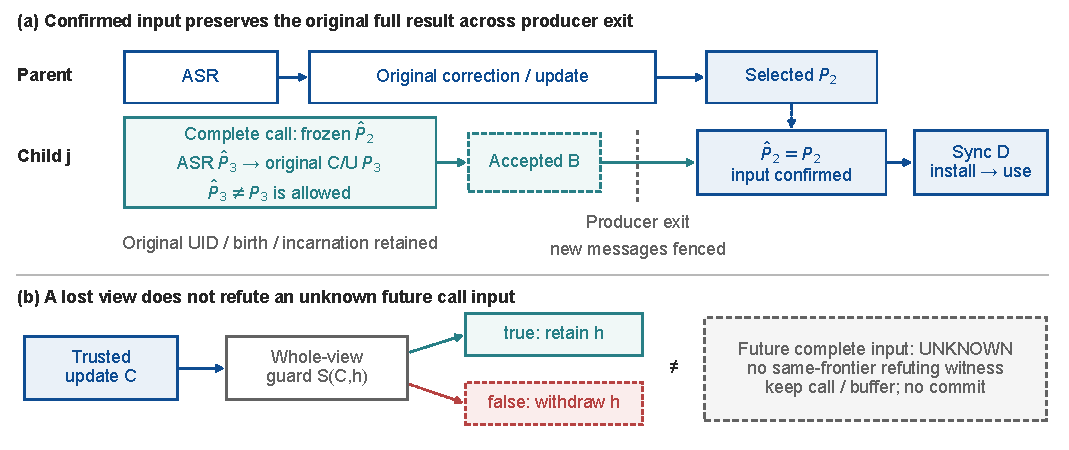
\includegraphics[width=\textwidth]{figures/coordination_protocol.pdf}
\caption{Eligibility, original selection, and whole-view support are
separate decisions. (a) A complete child call runs on frozen $\widehat P_2$;
its own prediction $\widehat P_3$ may differ from original C/U output $P_3$.
An accepted buffer keeps its original identity across producer exit and
fencing. Matching selected $P_2$ confirms the input; durable sync precedes
installation and use. (b) Losing view support does not refute an unknown
future input or authorize its commit. This is a causal native schematic,
with complete-state and execution assumptions from
Section~\ref{sec:contract}, not a measured timeline.}
\label{fig:protocol}
\end{figure*}

\subsection{Complete results and physical ownership}
In the core runtime, dispatch binds session,
incarnation, job, input, target, and contract. A row returns either a
complete result with re-derived state/text or cancellation without partial
state. Complete rows can be installed and consumed before their batch
finishes. Only all terminal rows and device synchronization authorize
\texttt{BatchDrained} and executor reuse. The native process lifecycle
below has separate evidence.

\subsection{Covered work and safe-point exit: \texorpdfstring{$K$}{K}}
For the tested use model, $K$ requests exit when the installed Canonical
frontier covers a proposal's target and it has no remaining declared use.
This differs from $R$: valid work beyond the new root can remain useful.
Workers observe \texttt{CancelRequest} at decode boundaries; completion
can win, but each row has one terminal outcome. Static batches are not
compacted or refilled; masked costs and drain delays remain measured.

\subsection{Durable facts and outstanding input}
Before acknowledgment, synchronized frames bind parent/next states,
request identity, selected complete result, and receipt; recorded deltas
must reconstruct the state. Group-ready commit shares synchronization
among validated sessions without a collection timeout or cross-session
atomic transaction. Uncertain append/application outcomes block writes.
Write-ahead recovery~\cite{mohan1992aries} reconstructs facts and identities;
the native extension binds this to original correction calls.

\subsection{Validation boundaries}
Propositions~\ref{prop:rebase} and~\ref{prop:continuity} concern the stated
guards and compatible applications. The artifact retains an earlier,
separately frozen recovery prototype and its bounded model and crash
results; they do not validate the later core or native fault paths.
The selected-trace argument of Proposition~\ref{prop:refinement}, its
finite specification, and actual execution checks have distinct scopes.

\subsection{Continuing through delivery and process failures}
\label{subsec:native_resilience}
Each job has an Owner namespace and monotonic issue number; each physical
slot has a worker incarnation, using established RPC identity principles
\cite{birrell1984rpc}. Fencing removes future message authority without
renaming already accepted complete results.

\paragraph{Local rejection and physical release}
The ingress guard rejects exact duplicates and fenced messages locally;
they cannot mutate selected state or release newer leases. Contradictory
currently owned contents freeze writes. Per-incarnation Pipes and receiver
threads isolate incomplete frames. Replacement requires process exit,
CUDA release and joined receivers. Strictly validate complete receipts
from the sealed channel before fencing the incarnation and retiring
unfinished work. Accepted buffers and supported views retain their
original identities.

\paragraph{Durable selection and recovery}
A synchronous hook binds complete parent/next states, original correction
and IDs, job, Owner/session epochs, and producer incarnation. Framing,
checksums and chaining protect the fact; synchronization precedes
installation/publication. Uncertain writes freeze the writer. Recovery
discards only an incomplete final frame; complete corruption fails.
These conventional write-ahead rules~\cite{mohan1992aries} bind the
original feedback transition.

The surviving Supervisor preserves the input ledger and original clocks.
After old physical ownership ends, it advances the Owner namespace,
replays the verified fact prefix, and cold-starts workers. Replay adds no
inference; old publications gain no new authority. Both policies share
this coordinator, durability, recovery, and actual Consumer.

\paragraph{Conditional continued service}
\phantomsection\label{prop:continued_service}
For finite accepted work after finite supported failures, further progress
requires readable storage, eventual physical release/loading, terminating
original calls that advance frontiers, fair Owner/Consumer scheduling,
and sufficient service budgets. This is not an RTO or D2/C8 guarantee;
loading, replay and recomputation retain their original clocks.

\paragraph{Control history}
Roots, calls, buffers, visible views and outboxes pin their dependencies.
Actual acknowledgment releases publication references, while the visible
view stays pinned. Namespace/issue high watermarks prevent reuse after
collection. Unreferenced terminal and audit windows have fixed limits;
diagnostics stream to disk. These bound protocol entries relative to live
dependencies, separately from current state, cumulative text and total
memory.

\section{Evaluation}\label{sec:eval}
\subsection{Experimental design and service endpoints}
We evaluate two service obligations under unchanged selected feedback
histories: retaining dependency-valid progress already at the Consumer,
and completing selected transitions before their original deadlines.
The core factorial study isolates computation and whole-view retention;
the native study tests input-confirmed full execution of the original
correction pipeline. Timing, content support, and energy remain separate.
The core experiments use actual neural
calls, durable input and Canonical journals, and an instrumented FIFO
Consumer. Measurements use Consumer applications rather than publication
or display replay. Accepted input obligations retain
their original arrival clocks.

\paragraph{Implementation and workloads}
The service uses two 24-GB RTX~3090s: an FP16 Private worker and an FP32
Authority worker. Qwen3-ASR~1.7B~\cite{shi2026qwen3asr} is the primary backend; Whisper base.en~\cite{radford2023whisper}
tests a second adapter. The common carrier uses complete-row delivery,
at most 16 rows per batch, a 256-token generation limit, the protocol
kernel, and synchronized journals. These experiments use
\texttt{row\_complete}: physical early exit is disabled, so the effects of
$R$ and $S$ cannot be attributed to cancellation. Model startup is outside
the serving interval and is recorded separately. Serving energy integrates
both physical boards; CPU energy is outside that measurement.

The independent confirmation comprises 24 previously unused speaker
streams from LibriSpeech~\cite{panayotov2015librispeech}, totaling
714.11~s, selected using metadata before inference and partitioned into
three eight-speaker cohorts. Its 110 cells contain 60 primary cells
(three cohorts, two backends, two arrival patterns, five arms), 20
fresh-process repeat cells on cohort~A, and 30 coarser-feedback controls.
Primary Authority advances at every 2-s input boundary ($\rho=1$);
$\rho=3$ changes both selection frequency and feedback segmentation.
Synchronized streams start together; staggered streams start 0.25~s
apart. Repeats and arms reuse these sources: the independent acoustic
sample is 24 speakers, not 110 deployments.

\paragraph{Comparators}
The four arms cross computation retention $R$ with whole-view retention
$S$ (Section~\ref{sec:continuation}). With $R$ disabled, computation
rebuilds from the selected root rather than retaining its witnessed
continuation. With $S$ disabled, a Canonical application replaces the
provisional view with the new certified snapshot. This
\emph{checked-snapshot} Consumer still validates Private dependencies
against the same root and passes the same protocol kernel. Removing
retention does not remove validation, durability, input accounting, or
the execution capability of Section~\ref{sec:protocol}.
The fifth arm, \emph{Full composition (ours)}, is a complete-composition
positive control: an alternative policy instantiation with the same
retention relation, Consumer protection, and shared execution/commit
substrate. It is neither an external pre-existing implementation of our
complete design nor an independently reimplemented neural stack.
Comparable behavior is the expected positive-control outcome.

\paragraph{Endpoints}
For offered interval $i$, let $w_i$ be its audio duration, $r_i$ its
original ready time, $d_i$ its first actual visible covering time, and
$c_i$ its first actual certified covering time. Original joint-deadline
credit is
\begin{equation}
 A_{2,8}=\sum_i w_i\,\mathbf{1}
 \{d_i-r_i\leq2\ \land\ c_i-r_i\leq8\}.
 \label{eq:credit}
\end{equation}
All offered audio, including end-of-stream (EOS) tails and misses, stays
in its denominator. Whole-run service passes only when display P99 is
at most 2~s and certified-view P99 at most 8~s. P99 is computed over
offered frontiers within each run; credit weights their audio durations.
Thus a P99 pass can coexist with a small tail miss. We separately measure
adjacent visible-frontier withdrawals, their audio magnitude, and the
integral of the deficit below the previously observed high watermark.
Text revisions, final word error rate (WER), and board energy remain
separate endpoints. Independent recounters check complete selected
$F/Z/P/\mathrm{text}$ histories and reconstruct dependency witnesses from
actual complete outputs and consumed inputs, rather than trusting a
retention flag.

\subsection{Does retained computation preserve delivered progress?}
We test whether preserving valid work also preserves its presentation when
selected updates replace snapshots.
Table~\ref{tab:core-h3} reports the pre-specified Qwen, $\rho=1$,
staggered stratum, including all three cohorts. Retaining computation
alone raises deadline credit from 654.115 to 664.150~s but increases
audio-frontier withdrawals from 12 to 17. The additional work survives
the new root, while snapshot consumption still discards its visible
progress. Retaining views alone reduces withdrawals to one but yields
628.435~s of credit. The joint arm obtains 680.760~s and zero
audio-frontier withdrawals: 26.645~s, or 3.73 percentage points of offered
audio, above $R_0S_0$. Its gain over computation-only
is 16.610~s.

\begin{table}[t]
\centering
\caption{Independent Qwen confirmation, $\rho=1$, staggered arrivals.
Each arm offers 714.11~s across three eight-speaker cohorts.
Withdrawals and credit are totals; P99 and energy are medians of three
per-run statistics. All 15 runs miss the whole-run D2 criterion.}
\label{tab:core-h3}
\begingroup
\small
\setlength{\tabcolsep}{3pt}
\begin{tabular}{@{}lrrrr@{}}
\toprule
Arm & \shortstack{Audio\\withdrawals} &
\shortstack{Display\\P99 (s)} & \shortstack{D2/C8\\credit (s)} &
\shortstack{Energy\\(J/audio-s)}\\
\midrule
$R_0S_0$ & 12 & 3.797 & 654.115 & 59.72\\
$R_0S_1$ & 1 & 3.891 & 628.435 & 59.16\\
$R_1S_0$ & 17 & 2.431 & 664.150 & 59.68\\
$R_1S_1$ & 0 & 2.329 & 680.760 & 59.37\\
Full (ours) & 0 & 2.534 & 667.530 & 59.73\\
\bottomrule
\end{tabular}
\endgroup
\end{table}

The cohort-wise credit interaction,
$I=Y_{11}-Y_{10}-Y_{01}+Y_{00}$, is
$+18.530$, $+6.205$, and $+17.555$~s. These three contrasts share queues
within each cohort. They support a composition effect
in this stratum, rather than treating individual deadline windows as
independent trials. The joint arm still erases 569 visible characters:
zero audio-frontier withdrawal does not mean immutable text.
Its 2.329-s median display P99 also remains above D2. The result preserves
more timely progress without establishing that this workload meets its
whole-run service target.

The full composition likewise has zero frontier withdrawals, the same 569
erased characters, and comparable timing and energy. Its lower credit
than the joint arm in this stratum is not evidence that a different
complete composition is inherently inferior. Across the confirmation,
all 144 matched source/backend/granularity/arrival history groups agree
on complete Canonical $F/Z/P/\mathrm{text}$; all 22 paired full-composition
comparisons preserve those histories. The ablations therefore isolate
how legal progress is retained, rather than buying latency by changing
the selected feedback task.
\emph{Lesson:} computation and consumption protect different objects;
their joint value is observed under the same selection contract.

\subsection{Relative progress explains when retention matters}
The useful opportunity is an already observed whole view ahead of a
new Canonical frontier whose complete dependency path remains valid.
In the headline joint arm, 18 of 368 Canonical updates encounter such
a view and retain it. Computation-only encounters 17 and clears all 17.
Under synchronized arrivals the joint arm encounters only three of
368; its credit is 0.790~s below computation-only. Without an ahead
view, preserving it has little service value. These are witnessed
incidences in the executed workload, not a production prevalence estimate.

Timing can also change the ranking. In the fresh-process staggered
repeat on cohort~A, joint credit is 226.320~s versus 230.565~s for
computation-only, and $I=-2.245$~s. We retain this repeat alongside
the three positive primary contrasts. The combination's value depends
on relative progress and actual feedback compatibility; independent
source confirmation does not imply an invariant timing advantage.

\subsection{When does retention become sustained service?}
We expect relative progress to determine both retention opportunities and
deadline outcomes. We freeze three development workloads---eight synchronized
sessions, eight staggered sessions, and sixteen staggered sessions---with
four arms and three fresh processes per arm (36 cells). A single later
exploratory midpoint adds twelve staggered sessions and the same twelve
arm/repeat cells. Figure~\ref{fig:service-region} retains all 48 runs.
The nested source lists offer 121.205, 185.300, and 250.180~s per
eight-, twelve-, and sixteen-session run. Adding sessions also adds
source content; these are explicit operating workloads, not a pure
concurrency capacity curve.

\begin{figure*}[t]
\centering
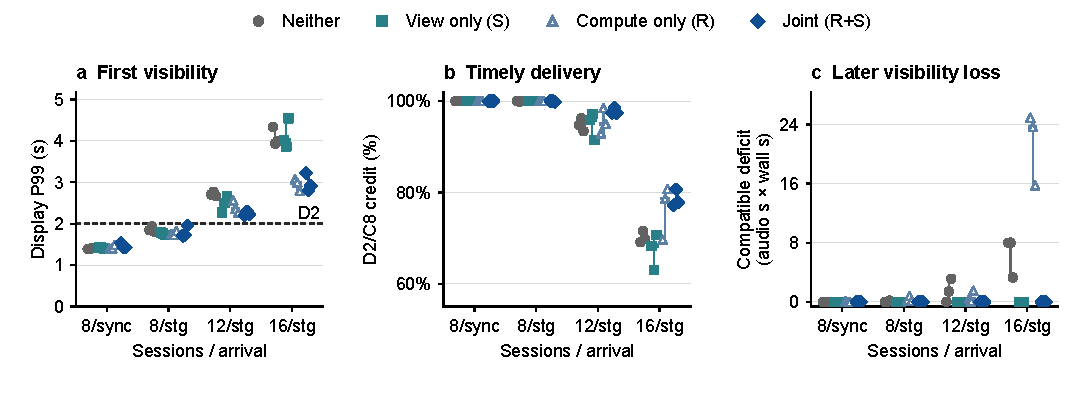
\includegraphics[width=\textwidth]{figures/service_region.pdf}
\caption{First visibility, timely credit, and later visibility loss are
different endpoints. All four workloads and three fresh runs per arm are
shown, including the negative twelve-session midpoint. Points are real
per-run values; ticks and ranges describe their median and observed
range. Panel~(c) is the separate secondary measure of subsequent
compatible loss of originally timely intervals, censored at the next
Canonical root when necessary. It does not replace panel~(b)'s original
first-observation credit.}
\label{fig:service-region}
\end{figure*}

All arms pass whole-run D2/C8 in the two eight-session workloads.
Joint display P99 is 1.426--1.528~s when synchronized, where the arms
largely converge. Staggered joint P99 reaches 1.955~s, and an earlier
development run reached 2.034~s, exposing a narrow timing margin.
Two 0.215-s tails exceed D2 in the new eight-session runs and remain
uncredited even though their runs' P99 passes. At sixteen sessions,
all twelve runs fail D2, while C8 passes. Joint credit exceeds $R_0S_0$
by 20.280/22.885/20.180~s, but its credit interactions are
$+20.910$, $+26.380$, and $-9.575$~s.
Against computation-only, joint credit changes by
$+18.910$, $+5.055$, and $-7.225$~s, and display P99 improves
in only one repeat. Continuity is the stable distinction: computation-only
withdraws compatible views 16/17/12 times, versus zero for joint.

First credit does not reveal a later withdrawal. A frozen secondary
recount therefore follows intervals already delivered within D2 whose
eventual certified covering view also meets C8. At each subsequent
Canonical application it classifies withdrawal using the complete old
view's dependency witness, separately recording necessary incompatible
withdrawals. Loss lasts until an actual covering view returns or the
next Canonical boundary censors this root's window. At sixteen sessions,
computation-only still has 10/12/9 timely compatible loss windows with
24.903/23.635/15.736 audio-s$\times$wall-s deficit area; joint has none.
Such holes intersect the original D2 read point for 6.000/10.675/4.000~s
of distinct audio. The secondary measures continuity after delivery;
it neither changes Eq.~\eqref{eq:credit} nor certifies provisional content.

The twelve-session witness is \emph{not established}: all twelve runs
fail D2, and computation-only never loses a timely complete non-EOS
interval satisfying the frozen witness criterion. Joint has no compatible
loss windows. The predeclared stop rule ends this search; full criteria
and per-run results remain in the artifact.
\emph{Lesson:} compatible retention prevents a specific later loss;
first-delivery performance and overload remain separate.

\subsection{Quality and cost boundaries}
All headline Qwen arms have WER $26/1908=1.36\%$ and identical selected
histories. Retrospective support counting first-certified content plus
first-ahead whole views that exactly match later same-$F$ Canonical
text leaves the headline credits unchanged. Elsewhere raw differences
remain: joint loses 2~s of strict support in the sixteen-session third
repeat and 2~s in each of the midpoint's first two repeats, although
the frozen text normalizer agrees. This comparison is with the selected
model output, not human-transcription correctness. Whisper exposes a
larger adapter boundary: WER is 83.12\% at $\rho=1$ and 11.53\% at
$\rho=3$, whose different feedback contract prevents interpreting it
as a quality-preserving speedup.

The headline arms consume similar board energy (Table~\ref{tab:core-h3});
energy does not rank them in credit order. At sixteen development
sessions, joint reduces total model time by 0.66--1.59~s against $R_0S_0$,
while serving wall time does not consistently fall and the
three energy differences change sign. The measured benefit is the
progress delivered and preserved under a fixed feedback contract.
It is not a general reduction in inference cost or a cure for overload.

\subsection{Do early full calls preserve the original task?}
\label{subsec:native_retention_eval}
We test whether input-confirmed calls improve service while retaining
original learned correction and recursive feedback. The StreamCorrect
adaptation uses fixed 500-ms inputs, no VAD, and original FP32 execution
\cite{vu2026streamcorrect}. Both author-built policies have two complete
workers, the same ASR early-view Consumer and neural warmup. Conservative
execution waits for selected parent feedback; Full-call permits conditional
execution. We distinguish the earlier implementation (\texttt{bdfa}) from
the final resilience implementation (\texttt{4f}); full execution identities
are in the artifact.

\paragraph{Independent confirmation and matched regression}
The earlier method was frozen before selecting four unused AISHELL-1
speakers~\cite{bu2017aishell} by metadata in an 8--9-s band. Two policies
and two fresh repeats give 16 runs with randomized pair blocks, reversed
arm order and swapped GPU roles. All selections, 500-ms frontiers and
partial EOS remain. Speakers, rather than repeated runs, are the acoustic
units. All 272 selected transitions match complete original start/end
states, correction and returned IDs against offline full-call references.
Both arms have five edits over 81 unique reference characters (6.17\%
CER); this is the adaptation's accuracy, not the published benchmark.
Earlier Full-call raises credit from 37.0 to 66.33975~s and passes
from 0/8 to 8/8.

\begin{table}[t]
\centering
\caption{Final full calls preserve task fidelity and improve timely
service. The matched version study reuses four measured speakers:
two policies, two versions and two fresh trials (32 runs). Each row offers
66.340~s; credit and energy are totals, D99 is the median of per-run P99.
Energy uses a common external origin-to-confirmed-physical-model-drain
window. This is regression evidence, not new acoustic confirmation.}
\label{tab:native_full_confirm}
\small\setlength{\tabcolsep}{2.5pt}
\begin{tabular}{@{}llrrrr@{}}
\toprule
Version & Policy & \shortstack{Credit\\(s)} & \shortstack{D99\\(s)} &
\shortstack{Energy\\(kJ)} & Pass\\
\midrule
Earlier & Conserv. & 33.500 & 4.450 & 44.690 & 0/8\\
Earlier & Full-call & 66.340 & 1.633 & 39.735 & 8/8\\
Final & Conserv. & 30.000 & 4.759 & 47.019 & 0/8\\
Final & Full-call & 65.822 & 1.638 & 43.952 & 6/8\\
\bottomrule
\end{tabular}
\end{table}

The matched 32-run study holds those four sources, FP32 models, warmup,
allocator and external board-power observation fixed across versions.
All 544 selected transitions match complete original inputs/outputs,
correction and IDs under the declared static code-version mapping.
Final Full-call earns 65.821625 versus 30.0~s and passes 6/8 versus 0/8
(Table~\ref{tab:native_full_confirm}). Its two failures are S0908 EOS:
display P99 increases by 0.163/0.050~s against Earlier Full-call.
Other paired differences have both signs; similar medians do not establish
equivalence. Final Full-call uses 6.52\% less drain-window board energy
than Final Conservative, but 10.61\% more than Earlier Full-call.
Model drain and source-specific cleanup are different endpoints;
EOS-window and original source endpoints remain separately available.

\paragraph{Resident independent requests}
Models load once per trial and both worker PIDs persist across four
pre-registered independent requests. The next request begins only after
actual certified consumption of the previous file EOS. This is
single-outstanding closed-loop service, without online VAD or open-arrival
capacity. Two policies and two fresh trials retain all 272 original
transitions and each request's own input clock. Full-call passes D2/C8 on
7/8 requests versus 0/8, earning 64.118875 versus 31.0 of 66.33975~s.
The second S0908 request has D99 2.229~s; residency does not remove its
deadline boundary.

\paragraph{What content arrives, and what remains?}
The earlier independent bank contains 92 promoted calls beginning before
their selected parent finishes; 20 have wrong own predicted ends.
Twenty-four invalid/covered calls stop after ASR and two complete
wrong-input results are discarded. Input confirmation, rather than
prediction correctness, explains which original work survives.

A frozen zero-neural recount of the final matched and resident logs
checks actual complete dependencies and first-view text at its own
frontier $G$. Credit whose whole first view retrospectively equals
selected text at that same $G$ rises from 22.5 to 51.0~s in matched runs,
and from 24.0 to 50.259~s in resident requests. Full-call's remaining
14.822/13.860~s mismatches; unknown coverage is zero. Raw and whitespace
comparisons agree. Each arm in either bank introduces 180 code-point
occurrences, retracts 14, and leaves 166 last-visible. All-offered
whole-text matches are 106/136 for Conservative and 104/136 for Full-call.
The gain is timely supported content, not more text or a higher overall
match fraction; agreement with selected model output is not human accuracy.

The final matched bank has no compatible-ahead application, so gives no
retention-rate evidence. Resident Full-call has one nonempty opportunity:
its 5.0-s whole view survives a compatible 4.5-s selected update with the
same tip and job. The complete tip is logically held for 0.817~s spanning
that update before legitimate supersession; this is Consumer event-state
observation, not avoided downtime. Each Full-call bank contains two
necessary incompatible withdrawals. Final objects are right-censored at
the last actual same-source observation. \emph{Lesson:} confirmed full
calls accelerate the original task, while content support, continuity
opportunities and deadline margin require their own denominators.

\subsection{What survives a producer or Owner failure?}
\label{subsec:same_source_validation}
We test whether failures preserve acquired results without granting old
messages new authority. The final implementation shares models,
durability, guards, recovery and Consumer across both policies. Initial
loading and fixed warmup precede service; replacement loading, replay,
recomputation and physical drain retain the original clock.

Six conditions, two policies and two fresh processes on one development
clip give 24 short trials, plus four EOS/compatible-view regressions.
With eight sustained-state trials below, the bank has 3,976 durable
transitions independently bound to original complete receipts and actual
Consumer applications: zero illegal installations or incorrect
owned-message rejections. Eight duplicate/late messages cause no selected
mutation; eight worker deaths have confirmed physical replacements.
Conditional calls supply 354 durable facts: 352 have original Owner
installation records, and two first reach the Consumer through recovery.
In four worker-after-ASR cases, an already consumed whole view remains
across producer exit/fencing until legitimate correction. This is retained
Consumer state, not redelivery or proof that the prediction was correct.

\begin{table*}[t]
\centering
\caption{Fault containment preserves legality, while cold recovery misses
the original service deadlines. Six short conditions use one fixed clip
and two fresh trials per policy. Each cell lists Conservative above
Full-call; ranges are observed minima/maxima. Illegal; done gives illegal
installations and completed/2 trials. Reject/mutation counts local
rejections and selected changes. New result is fault-to-actual-certified
consumption of a new fact whose call completes after the fault, excluding
old-fact replay and replacement readiness. D2/C8 counts joint whole-run
passes; EOS counts D2 misses. Both-board energy runs through physical drain.}
\label{tab:native_reliability}
\begingroup\fontsize{8.5}{10}\selectfont
\setlength{\tabcolsep}{3pt}
\begin{tabular}{lrrrrrr}
\toprule
Condition & Illegal; done & Reject / mutation & New result (s) & D2/C8 pass & EOS miss & Energy (J) \\
\midrule
No fault & \shortstack{0; 2/2\\0; 2/2} & \shortstack{0 / 0\\0 / 0} & \shortstack{--\\--} & \shortstack{0/2\\1/2} & \shortstack{2\\1} & \shortstack{6566--6574\\5896--5911} \\
Duplicate / late & \shortstack{0; 2/2\\0; 2/2} & \shortstack{4 / 0\\4 / 0} & \shortstack{--\\--} & \shortstack{0/2\\1/2} & \shortstack{2\\1} & \shortstack{5701--5893\\5538--5846} \\
Worker after ASR & \shortstack{0; 2/2\\0; 2/2} & \shortstack{0 / 0\\0 / 0} & \shortstack{1.90--2.22\\2.15--2.21} & \shortstack{0/2\\0/2} & \shortstack{2\\2} & \shortstack{5182--5401\\5447--5647} \\
Worker partial frame & \shortstack{0; 2/2\\0; 2/2} & \shortstack{0 / 0\\0 / 0} & \shortstack{2.10--2.25\\1.76--2.23} & \shortstack{0/2\\0/2} & \shortstack{2\\2} & \shortstack{4775--5178\\5492--5594} \\
Owner before durable & \shortstack{0; 2/2\\0; 2/2} & \shortstack{0 / 0\\0 / 0} & \shortstack{86.42--108.08\\64.61--107.09} & \shortstack{0/2\\0/2} & \shortstack{2\\2} & \shortstack{24549--28019\\19571--26557} \\
Owner after durable & \shortstack{0; 2/2\\0; 2/2} & \shortstack{0 / 0\\0 / 0} & \shortstack{83.90--87.05\\101.80--104.44} & \shortstack{0/2\\0/2} & \shortstack{2\\2} & \shortstack{22415--24200\\26483--27171} \\
\bottomrule
\end{tabular}
% Fixed vertical order within each cell: Conservative / Full-call. Ranges are two fresh trials, not confidence intervals.
% New result copies frozen 4f fault_to_new_certified_result (runtime model_end>=fault filter). Any strict > statement is a separately audited observed property.
% A qualifying call may already be in flight on a surviving worker. This clock is neither replacement-neural readiness nor old durable replay.
% Illegal installs require independent trace-checker evidence. ? means unknown. -- means not applicable, not zero.
% Main table: development S0908 24 cells only. Regression4 and sustained8 remain separately listed in ALL36_MACHINE_TABLE.

\endgroup
\end{table*}

Table~\ref{tab:native_reliability} keeps all deadline failures. Normal and
duplicate Full-call each pass one of two trials; the other misses D2 only
at EOS. All worker-fault trials fail D2 but pass C8; Owner-fault trials
fail both. Old durable facts reappear in 1.36--1.81~s, while new certified
post-fault completions take 64.61--108.08~s in Owner cases. A surviving
worker may finish before replacement readiness. Old-fact replay and new
inference are separate recovery endpoints.

\paragraph{Complete buffers across producer death}
The bank above never installs a completed conditional buffer. Four frozen
timing controls cover two matching and two mismatching inputs. A transport
fixture holds the parent after original ASR and the child after sending
its complete original result. After the Owner registers the result, we
kill its producer, verify exit, CUDA release, sealed-channel validation
and fencing, then release original parent correction. Both matching
results install and are consumed once with their original job, birth and
incarnation; both mismatches are rejected against the actual same-frontier
parent. Positive cases also finish a subsequent independent request.
These are controlled interleavings, not natural incidence or fault-time
SLO wins. A separately frozen zero-neural reconstruction validates the
unchanged runs after correcting a READY indexing defect; original failed
audit gates remain in the artifact. \emph{Lesson:} producer failure ends
future message authority without uniformly invalidating accepted results.

\paragraph{Sustained-state stress and its limits}
Two metadata-selected AISHELL-1 speakers contribute 24 utterances each,
concatenated as exact PCM into 228.51025/208.1003125-s streams without
join resets. A continuous original-engine reference and 875 separately
restored steps agree on complete state, correction and IDs, crossing
398/357 buffer shifts and 353/252 context changes. Eight serving trials
produce 3,500 matching selected steps. Unpinned terminal and each audit
class stay at most 64 entries; live dependencies, state/output bytes,
Owner RSS and cumulative logs are separate.

All eight trials fail D2/C8 (display P99 449.727--502.952~s). Both policies
reproduce severe original-task insertion errors: CER 3103/486 (638.48\%)
and 1313/522 (251.53\%). Full-call uses more energy. The original length
guard can skip decoding, so frontier credit need not add text. These are
state/collection stress tests, not deployable continuous ASR. Across all
36 trials, the checker preserves 90 compatible-ahead dependency-tip
applications and records 1,118 necessary incompatible withdrawals. Internal
tips need not add text; these controlled counts do not estimate natural
prevalence.

An independent dispatch audit finds 360 eventual matches among 1,901
conditional inputs; 1,541 are refuted, none unresolved. Six matched jobs
never become durable after injected failures. Workload-specific ratios
remain separate. Original-clock misses and a conservative offline
excess-length bound precede the after-trim 448-token condition on each
long stream; neither yields online prefix CER or a unique causal diagnosis.

% Compressed earlier K24 support; full measured ledger remains in the artifact.
% This core execution evidence is separate from native failure validation.
\subsection{From physical release to supported service}
\label{subsec:release_evidence}
A separate 24-run core study crosses $R$ and $K$ with $S$ enabled,
two arrival patterns and three fresh processes, using a frozen
wrong-conditioning fixture. Selected histories and WER $14/687$ match;
all 675 same-input/prompt/audio/peer-order pairs return identical outputs.
Synchronized $R1$ releases the next 16-row computation 473--577\,ms
earlier. All 96 following rows are actually consumed and their whole
texts match later same-frontier Canonical text. Only 6/6/1 rows switch
from deadline miss to hit. Adding $K$ changes credit by +7.970 to
+15.255\,s when synchronized and $-26.000$ to $+21.780$\,s when
staggered, without consistent energy savings. Request acknowledgment
still precedes physical drain. This is a measured release-to-service
opportunity, with no stable positive $R\times K$ interaction.


\section{Related Work}\label{sec:related}
\paragraph{Incremental information and dependency reuse}
The incremental-unit model separates newest committed information from
the active right edge and propagates dependency revocation
\cite{schlangen2011incremental}. Its commit promises that a unit will not
be revoked. Here, certification records acceptance by the protected
selection protocol; later selected facts may still revise the transcript.
Adapton checks recorded dependencies; Nominal Adapton combines names with
arguments and dependency checks to recover reusable work
\cite{hammer2014adapton,hammer2015names}. Differential Dataflow maintains
incremental computations across evolving versions
\cite{mcsherry2013differential}. These works establish much of the basis for
dependency-aware reuse. RevTrace instantiates that basis for complete
neural feedback state and frozen executed calls. Its service obligation
connects execution eligibility to the actual whole view retained when an
independently selected root is applied.
Our sufficient witness follows recorded executions; it does not transfer a
from-scratch theorem to independently repeated floating-point inference.

\paragraph{Revisable speech services and speculation}
Whisper-Streaming converts an offline recognizer into incremental service
using LocalAgreement~\cite{machacek2023whisperstreaming}. StreamCorrect
adds learned correction and feeds selected corrections into subsequent
recognition~\cite{vu2026streamcorrect}. RevTrace retains that selection and
feedback behavior in its controlled native adapter; its contribution
concerns the asynchronous execution and consumption around the feedback
boundary. It does not introduce a better acoustic model or train a new
corrector.

SSBD coordinates old-output draft reuse with display-only suffix masking
\cite{zeng2026ssbd}. It revalidates a draft under updated input and includes
an unbiased configuration. RevTrace follows complete calls that actually
executed to establish their eligibility under newly selected feedback state,
then checks the dependency witness for the Consumer's whole current view.
PredGen provides a close precedent for speculation while speech input
evolves across recognition, language generation, and speech synthesis
\cite{li2025predgen}. Our comparison holds the complete selected feedback
task fixed across the retention policies. The specific reuse object,
protected selection, and whole-view transition define the composition
evaluated here. RelayS2S uses a learned verifier to commit a fast-path
prefix that constrains subsequent slow-path generation
\cite{mai2026relays2s}. Our native calls instead confirm their complete
inputs and retain the original correction and feedback update. Work on
ASR alignment drift also establishes the importance and cost of audio
position state~\cite{wang2026alignmentdrift}; our contract includes that
state rather than treating text equality as sufficient.

\paragraph{Execution, authorization, and recovery}
Retire jointly addresses revocation, valid state inheritance and physical
reclamation for runtime-selected version transitions~\cite{zhang2026retire}.
RevTrace derives complete-call eligibility and whole-view actions from
an unchanged selected feedback task: an unsupported view can be withdrawn
while a future call's input remains unresolved. Our covered-exit policy
is execution support, without a new general cancellation claim. The
parent-version control does not reproduce the complete Retire system.

Optimistic and multiversion concurrency control separate validation and
commit from concurrent execution~\cite{kung1981occ,bernstein1983mvcc}.
Write-ahead recovery persists state changes and identities
\cite{mohan1992aries}, and stream-processing systems coordinate recoverable
state~\cite{carbone2017flinkstate}. We use these established principles at
the ASR feedback boundary. They supply machinery for ordering and
durability; the adapter still has to specify which state constitutes a
valid continuation and which complete view the Consumer may retain.

\section{Discussion}\label{sec:discussion}
\paragraph{Scope of the guarantee}
The continuation witness assumes a sufficient adapter state and faithful
execution of frozen inputs. A new adapter must account for every mutable
field that can affect later inference, selection, or feedback. A hidden
KV cache, alignment cursor, or external tool state can invalidate a
token-only argument. Conservative rejection remains allowed when a
sufficient witness is absent. The guarantee concerns dependency validity
and an individual compatible application; it supplies neither transcription
correctness nor monotone text for an entire session.

\paragraph{Progress, content, and capacity}
Processing more audio can leave the cumulative transcript unchanged.
Frontier credit, actual text additions and revisions, eventual selected
text agreement, and ground-truth accuracy answer different questions. We
report them with their original denominators. Preserving compatible
progress also cannot remove all input synchronization, queueing, or neural
work. The negative c12 witness identifies a timing boundary. An earlier
native two-source test earns 17.0~s with retention versus 18.5~s for
independent full replicas, at higher energy and a different warmup/Consumer.
These do not define a universal capacity envelope. Independent native
confirmation establishes a
single-chain service opportunity with the original selected task; it
does not turn that result into saturated multi-source capacity.

\paragraph{Deployment and validation}
The continuous-original reference exercises the native cut across real
buffer and context changes; another adapter must establish its own state
sufficiency. Active-dependency collection bounds protocol entries relative
to live references, separately from cumulative text, current state, and
total memory. Owner/worker recovery assumes the surviving services of
Section~\ref{sec:contract}. Replaying old facts restores access to that
prefix; the measured cold Owner restarts still miss original deadlines
for new work. Broader ownership transfer requires separate validation.
Finite specifications, source controls, controlled faults, actual GPU
service, and retrospective checks provide distinct evidence.

\paragraph{Eligibility and resource admission}
A valid input witness determines whether an owned call may be used.
It does not determine whether starting another conditional call is
worthwhile. Limiting new speculation can leave existing supported whole
views intact. The long stress study motivates this separate resource
decision. In a bounded two-client probe, new speculative calls precede
another client's ready necessary call in both repeats. The later client
has no additional C8 misses, and its C99 penalty fails the predeclared
repeat-consistency gate. No admission controller or general native-session
fairness is evaluated.

% Keep the conclusion opening together in the final technical-page column.
\newpage
\section{Conclusion}\label{sec:conclusion}
RevTrace separates complete-input eligibility, original selection authority,
and whole-view support while trusted feedback advances. Service experiments
expose a coordination gap: first delivery can meet its deadline, yet a
compatible update can withdraw that progress. The joint design protects
the supported ahead view. Native full calls can retain original correction
work after their inputs are confirmed even when their own next predictions
are wrong. Durable facts and physical identities carry this distinction
through supported process failures. The resulting composition connects
dependency reuse to actual continued consumption under a fixed feedback
task. Computation-only retention increases frontier withdrawals in the
headline factorial stratum; joint retention prevents them. Final native
calls improve timely supported-content credit while keeping necessary
revisions and EOS misses. Actual support, timing, recovery and capacity
bound the composition's benefit.
Extending recovery to Supervisor failure remains a separate direction.

\section*{AI Tool Usage}
ChatGPT/Codex assisted literature discovery, drafting and revision of all
manuscript sections and the refinement argument, runtime extensions and
experiment orchestration, and validation/analysis code producing the
figures and tables from recorded measurements. The artifact records
execution sources, frozen configurations, controls, and result provenance,
separating actual service measurements from component tests and
retrospective analyses. Constructed streams concatenate recorded AISHELL-1
PCM. The authors retain responsibility for the submission.
\clearpage
\bibliographystyle{IEEEtran}
\bibliography{refs,formal_refs,coordination_refs}
\end{document}
